\documentclass[11pt,fleqn, openany]{book} % Default font size and left-justified equations

%%%%%%%%%%%%%%%%%%%%%%%%%%%%%%%%%%%%%%%%%
% The Legrand Orange Book
% Structural Definitions File
% Version 2.1 (26/09/2018)
%
% Original author:
% Mathias Legrand (legrand.mathias@gmail.com) with modifications by:
% Vel (vel@latextemplates.com)
% 
% This file was downloaded from:
% http://www.LaTeXTemplates.com
%
% License:
% CC BY-NC-SA 3.0 (http://creativecommons.org/licenses/by-nc-sa/3.0/)
%
%%%%%%%%%%%%%%%%%%%%%%%%%%%%%%%%%%%%%%%%%

%----------------------------------------------------------------------------------------
%	VARIOUS REQUIRED PACKAGES AND CONFIGURATIONS
%----------------------------------------------------------------------------------------

\usepackage[table]{xcolor}

\usepackage{graphicx}
\usepackage{tabularx} % Required for including pictures
\usepackage{pgf,tikz,tkz-tab,eurosym,yhmath, stmaryrd}
\usepackage{pgfplots}
\usepackage{mathrsfs}
\usetikzlibrary{patterns}
\usetikzlibrary{trees}
\graphicspath{{../../Pictures/}}
\usepackage{multicol} 


\usepackage[english]{babel} % English language/hyphenation
\usepackage{icomma}
\usepackage{enumitem} % Customize lists
\setlist{nolistsep, nosep, nolistsep} % Reduce spacing between bullet points and numbered lists

\usepackage{booktabs} % Required for nicer horizontal rules in tables

 % Required for specifying colors by name


\definecolor{ocre}{RGB}{243,102,25} % Define the orange color used for highlighting throughout the book

\usepackage{listings}

\definecolor{codegreen}{rgb}{0,0.6,0}
\definecolor{codegray}{rgb}{0.5,0.5,0.5}
\definecolor{codepurple}{rgb}{0.58,0,0.82}
\definecolor{backcolour}{rgb}{0.95,0.95,0.92}

\lstdefinestyle{mystyle}{
    backgroundcolor=\color{backcolour},   
    commentstyle=\color{codegreen},
    keywordstyle=\color{magenta},
    numberstyle=\tiny\color{codegray},
    stringstyle=\color{codepurple},
    basicstyle=\ttfamily\footnotesize,
    breakatwhitespace=false,         
    breaklines=true,                 
    captionpos=b,                    
    keepspaces=true,                 
    numbers=left,                    
    numbersep=5pt,                  
    showspaces=false,                
    showstringspaces=false,
    showtabs=false,                  
    tabsize=2
}

\lstset{style=mystyle}

%----------------------------------------------------------------------------------------
% Paramétrage XSIM
%----------------------------------------------------------------------------------------

\usepackage[no-files]{xsim}


\DeclareExerciseEnvironmentTemplate{myex}{%
    \textbf{%
      \hypertarget{ex:\ExerciseID}{\sffamily{\ensuremath{\blacktriangleright}} Exercice \GetExerciseProperty{counter} \GetExerciseProperty{subtitle} --}
      \hyperlink{sol:\ExerciseID}{Voir le corrigé}%
    }\par
}{\par\smallskip}

\DeclareExerciseEnvironmentTemplate{mysol}{%
    \textbf{%
      \hypertarget{sol:\ExerciseID}{\sffamily{\ensuremath{\blacktriangleright}} Correction \GetExerciseProperty{counter} --}
      \hyperlink{ex:\ExerciseID}{Voir l'énoncé}%
    }\par
}{\par\medskip}

\xsimsetup{
  exercise/template = myex ,
  solution/template = mysol 
}

%Collection exercices

\DeclareExerciseTagging{topic}

\xsimsetup{collect}

%----------------------------------------------------------------------------------------
% SYMBOLES
%----------------------------------------------------------------------------------------

\newcommand\imCMsym[4][\mathord]{%
  \DeclareFontFamily{U} {#2}{}
  \DeclareFontShape{U}{#2}{m}{n}{
    <-6> #25
    <6-7> #26
    <7-8> #27
    <8-9> #28
    <9-10> #29
    <10-12> #210
    <12-> #212}{}
  \DeclareSymbolFont{CM#2} {U} {#2}{m}{n}
  \DeclareMathSymbol{#4}{#1}{CM#2}{#3}
}
\newcommand\alsoimCMsym[4][\mathord]{\DeclareMathSymbol{#4}{#1}{CM#2}{#3}}

\imCMsym{cmmi}{124}{\CMjmath}

\newcommand{\Oij}{(O\,;\,\vec{\imath}\,,\, \vec{\CMjmath} )}
\newcommand{\Oijk}{(O\,;\,\vec{\imath}\,,\, \vec{\CMjmath}\,,\,\vec{k})}

\newcommand\e{\mathrm{e}}
\newcommand\R{\mathbb{R}}
\newcommand\N{\mathbb{N}}


%----------------------------------------------------------------------------------------
%	MARGINS
%----------------------------------------------------------------------------------------

\usepackage{geometry} % Required for adjusting page dimensions and margins

\geometry{
	paper=a4paper, % Paper size, change to letterpaper for US letter size
	top=3cm, % Top margin
	bottom=3cm, % Bottom margin
	left=2cm, % Left margin
	right=2cm, % Right margin
	headheight=14pt, % Header height
	footskip=1.4cm, % Space from the bottom margin to the baseline of the footer
	headsep=10pt, % Space from the top margin to the baseline of the header
	%showframe, % Uncomment to show how the type block is set on the page
}

\setlength{\parindent}{0pt}
\parskip=5pt



%----------------------------------------------------------------------------------------
%	FONTS
%----------------------------------------------------------------------------------------

\usepackage{avant} % Use the Avantgarde font for headings
\usepackage{times} % Use the Times font for headings
\usepackage{mathptmx} % Use the Adobe Times Roman as the default text font together with math symbols from the Sym­bol, Chancery and Com­puter Modern fonts

%\usepackage{microtype} % Slightly tweak font spacing for aesthetics
%\usepackage[utf8]{inputenc} % Required for including letters with accents
\usepackage[T1]{fontenc} % Use 8-bit encoding that has 256 glyphs

%----------------------------------------------------------------------------------------
%	BIBLIOGRAPHY AND INDEX
%----------------------------------------------------------------------------------------

\usepackage[style=numeric,citestyle=numeric,sorting=nyt,sortcites=true,autopunct=true,babel=hyphen,hyperref=true,abbreviate=false,backref=true,backend=biber]{biblatex}
\addbibresource{bibliography.bib} % BibTeX bibliography file
\defbibheading{bibempty}{}

\usepackage{calc} % For simpler calculation - used for spacing the index letter headings correctly
\usepackage{makeidx} % Required to make an index
\makeindex % Tells LaTeX to create the files required for indexing

%----------------------------------------------------------------------------------------
%	MAIN TABLE OF CONTENTS
%----------------------------------------------------------------------------------------

\usepackage{titletoc} % Required for manipulating the table of contents

\contentsmargin{0cm} % Removes the default margin

% Part text styling (this is mostly taken care of in the PART HEADINGS section of this file)
\titlecontents{part}
	[0cm] % Left indentation
	{\addvspace{20pt}\bfseries} % Spacing and font options for parts
	{}
	{}
	{}

% Chapter text styling
\titlecontents{chapter}
	[1.25cm] % Left indentation
	{\addvspace{12pt}\large\sffamily\bfseries} % Spacing and font options for chapters
	{\color{ocre!60}\contentslabel[\Large\thecontentslabel]{1.25cm}\color{ocre}} % Formatting of numbered sections of this type
	{\color{ocre}} % Formatting of numberless sections of this type
	{\color{ocre!60}\normalsize\;\titlerule*[.5pc]{.}\;\thecontentspage} % Formatting of the filler to the right of the heading and the page number

% Section text styling
\titlecontents{section}
	[1.25cm] % Left indentation
	{\addvspace{3pt}\sffamily\bfseries} % Spacing and font options for sections
	{\contentslabel[\thecontentslabel]{1.25cm}} % Formatting of numbered sections of this type
	{} % Formatting of numberless sections of this type
	{\hfill\color{black}\thecontentspage} % Formatting of the filler to the right of the heading and the page number

% Subsection text styling
\titlecontents{subsection}
	[1.25cm] % Left indentation
	{\addvspace{1pt}\sffamily\small} % Spacing and font options for subsections
	{\contentslabel[\thecontentslabel]{1.25cm}} % Formatting of numbered sections of this type
	{} % Formatting of numberless sections of this type
	{\ \titlerule*[.5pc]{.}\;\thecontentspage} % Formatting of the filler to the right of the heading and the page number

% Figure text styling
\titlecontents{figure}
	[1.25cm] % Left indentation
	{\addvspace{1pt}\sffamily\small} % Spacing and font options for figures
	{\thecontentslabel\hspace*{1em}} % Formatting of numbered sections of this type
	{} % Formatting of numberless sections of this type
	{\ \titlerule*[.5pc]{.}\;\thecontentspage} % Formatting of the filler to the right of the heading and the page number

% Table text styling
\titlecontents{table}
	[1.25cm] % Left indentation
	{\addvspace{1pt}\sffamily\small} % Spacing and font options for tables
	{\thecontentslabel\hspace*{1em}} % Formatting of numbered sections of this type
	{} % Formatting of numberless sections of this type
	{\ \titlerule*[.5pc]{.}\;\thecontentspage} % Formatting of the filler to the right of the heading and the page number

%----------------------------------------------------------------------------------------
%	MINI TABLE OF CONTENTS IN PART HEADS
%----------------------------------------------------------------------------------------

% Chapter text styling
\titlecontents{lchapter}
	[0em] % Left indentation
	{\addvspace{15pt}\large\sffamily\bfseries} % Spacing and font options for chapters
	{\color{ocre}\contentslabel[\Large\thecontentslabel]{1.25cm}\color{ocre}} % Chapter number
	{}  
	{\color{ocre}\normalsize\sffamily\bfseries\;\titlerule*[.5pc]{.}\;\thecontentspage} % Page number

% Section text styling
\titlecontents{lsection}
	[0em] % Left indentation
	{\sffamily\small} % Spacing and font options for sections
	{\contentslabel[\thecontentslabel]{1.25cm}} % Section number
	{}
	{}

% Subsection text styling (note these aren't shown by default, display them by searchings this file for tocdepth and reading the commented text)
\titlecontents{lsubsection}
	[.5em] % Left indentation
	{\sffamily\footnotesize} % Spacing and font options for subsections
	{\contentslabel[\thecontentslabel]{1.25cm}}
	{}
	{}

%----------------------------------------------------------------------------------------
%	HEADERS AND FOOTERS
%----------------------------------------------------------------------------------------


\usepackage{fancyhdr} % Required for header and footer configuration

\pagestyle{fancy}
\renewcommand{\chaptermark}[1]{\markboth{\sffamily\normalsize\bfseries\ \thechapter.\ #1}{}} % Chapter text font settings
\renewcommand{\sectionmark}[1]{\markright{\sffamily\normalsize\thesection\hspace{5pt}#1}{}} % Section text font settings
\fancyhf{} \fancyhead[LE,RO]{\sffamily\normalsize\thepage} % Font setting for the page number in the header
\fancyhead[LO]{\rightmark} % Print the nearest section name on the left side of odd pages
\fancyhead[RE]{\leftmark} % Print the current chapter name on the right side of even pages

\fancyfoot[L]{Jason LAPEYRONNIE}
\fancyfoot[R]{\href{http://mathoutils.fr}{http://mathoutils.fr}} % Uncomment to include a footer

\renewcommand{\headrulewidth}{0.5pt} % Thickness of the rule under the header
\renewcommand{\footrulewidth}{0.5pt} % Thickness of the rule under the header

\fancypagestyle{plain}{% Style for when a plain pagestyle is specified
	\fancyhead{}\renewcommand{\headrulewidth}{0pt}%
}

% Removes the header from odd empty pages at the end of chapters
\makeatletter
\renewcommand{\cleardoublepage}{
\clearpage\ifodd\c@page\else
\hbox{}
\vspace*{\fill}
\thispagestyle{empty}
\newpage
\fi}

%----------------------------------------------------------------------------------------
%	THEOREM STYLES
%----------------------------------------------------------------------------------------

\usepackage{amsmath,amsfonts,amssymb,amsthm} % For math equations, theorems, symbols, etc

\newcommand{\intoo}[2]{\mathopen{]}#1\,;#2\mathclose{[}}
\newcommand{\ud}{\mathop{\mathrm{{}d}}\mathopen{}}
\newcommand{\intff}[2]{\mathopen{[}#1\,;#2\mathclose{]}}
\renewcommand{\qedsymbol}{$\blacksquare$}
\newtheorem{notation}{Notation}[section]

% Boxed/framed environments
\newtheoremstyle{ocrenumbox}% Theorem style name
{0pt}% Space above
{0pt}% Space below
{\normalfont}% Body font
{}% Indent amount
{\small\bf\sffamily\color{ocre}}% Theorem head font
{\;:\;}% Punctuation after theorem head
{0.25em}% Space after theorem head
{\small\sffamily\color{ocre}\thmname{#1}\nobreakspace\thmnumber{\@ifnotempty{#1}{}\@upn{#2}}% Theorem text (e.g. Theorem 2.1)
\thmnote{\nobreakspace\the\thm@notefont\sffamily\bfseries\color{black}---\nobreakspace#3}} % Optional theorem note

\newtheoremstyle{blacknumex}% Theorem style name
{5pt}% Space above
{10pt}% Space below
{\normalfont}% Body font
{} % Indent amount
{\small\bf\sffamily}% Theorem head font
{\;:\;}% Punctuation after theorem head
{0.25em}% Space after theorem head
{\small\sffamily{\tiny\ensuremath{\blacksquare}}\nobreakspace\thmname{#1}\nobreakspace\thmnumber{\@ifnotempty{#1}{}\@upn{#2}}% Theorem text (e.g. Theorem 2.1)
\thmnote{\nobreakspace\the\thm@notefont\sffamily\bfseries---\nobreakspace#3}}% Optional theorem note

\newtheoremstyle{blacknumexo}% Theorem style name
{15pt}% Space above
{10pt}% Space below
{\normalfont}% Body font
{} % Indent amount
{\small\bf\sffamily}% Theorem head font
{}% Punctuation after theorem head
{0.5em}% Space after theorem head
{\small\sffamily{\ensuremath{\blacktriangleright}}\nobreakspace\thmname{#1}\nobreakspace\thmnumber{\@ifnotempty{#1}{}\@upn{#2}}% Theorem text (e.g. Theorem 2.1)
\thmnote{\nobreakspace\the\thm@notefont\sffamily\bfseries---\nobreakspace#3} \\}% Optional theorem note



\newtheoremstyle{blacknumbox} % Theorem style name
{0pt}% Space above
{5pt}% Space below
{}% Body font
{}% Indent amount
{\large\bf\sffamily}% Theorem head font
{\;:\;}% Punctuation after theorem head
{0.25em}% Space after theorem head
{\small\sffamily\thmname{#1}\nobreakspace\thmnumber{\@ifnotempty{#1}{}\@upn{#2}}% Theorem text (e.g. Theorem 2.1)
\thmnote{\nobreakspace\the\thm@notefont\sffamily\bfseries---\nobreakspace#3}}% Optional theorem note

% Non-boxed/non-framed environments
\newtheoremstyle{ocrenum}% Theorem style name
{5pt}% Space above
{5pt}% Space below
{\normalfont}% Body font
{}% Indent amount
{\small\bf\sffamily\color{ocre}}% Theorem head font
{\;:\;}% Punctuation after theorem head
{0.25em}% Space after theorem head
{\small\sffamily\color{ocre}\thmname{#1}\nobreakspace\thmnumber{\@ifnotempty{#1}{}\@upn{#2}}% Theorem text (e.g. Theorem 2.1)
\thmnote{\nobreakspace\the\thm@notefont\sffamily\bfseries\color{black}---\nobreakspace#3}} % Optional theorem note
\makeatother

% Defines the theorem text style for each type of theorem to one of the three styles above
\newcounter{dummy} 
\newcounter{thm}
\newcounter{correction}
\newcounter{qst}
\theoremstyle{ocrenumbox}
\newtheorem{theoremeT}[dummy]{Théorème}
\newtheorem{exerciseT}{Propriété}
\newtheorem{principeT}{Principe}
\theoremstyle{blacknumex}
\newtheorem{exampleT}{Exemple}
\theoremstyle{blacknumexo}
\newtheorem{exo}[thm]{Exercice}
\newtheorem{corr}[correction]{Correction}
\newtheorem{quest}[qst]{Question}
\theoremstyle{blacknumbox}
\newtheorem{vocabulary}{Vocabulary}[section]
\newtheorem{definitionT}{Définition}
\newtheorem{corollaryT}[dummy]{Corollary}
\theoremstyle{ocrenum}
\newtheorem{proofT}[dummy]{Démonstration}


%----------------------------------------------------------------------------------------
%	DEFINITION OF COLORED BOXES
%----------------------------------------------------------------------------------------

\RequirePackage[framemethod=default]{mdframed} % Required for creating the theorem, definition, exercise and corollary boxes

% Theorem box
\newmdenv[skipabove=7pt,
skipbelow=7pt,
backgroundcolor=black!5,
linecolor=ocre,
innerleftmargin=5pt,
innerrightmargin=5pt,
innertopmargin=10pt,
leftmargin=0cm,
rightmargin=0cm,
innerbottommargin=5pt]{tBox}

%Proposition box	  
\newmdenv[skipabove=7pt,
skipbelow=7pt,
rightline=false,
leftline=true,
topline=false,
bottomline=false,
backgroundcolor=ocre!10,
linecolor=ocre,
innerleftmargin=5pt,
innerrightmargin=5pt,
innertopmargin=10pt,
innerbottommargin=3pt,
leftmargin=0cm,
rightmargin=0cm,
linewidth=4pt]{eBox}	

% Definition box
\newmdenv[skipabove=7pt,
backgroundcolor=ocre!4,
skipbelow=7pt,
rightline=false,
leftline=true,
topline=false,
bottomline=false,
linecolor=ocre,
innerleftmargin=5pt,
innerrightmargin=5pt,
innertopmargin=10pt,
leftmargin=0cm,
rightmargin=0cm,
linewidth=4pt,
innerbottommargin=5pt]{dBox}	

% Corollary box
\newmdenv[skipabove=7pt,
skipbelow=7pt,
rightline=false,
leftline=true,
topline=false,
bottomline=false,
linecolor=gray,
backgroundcolor=black!5,
innerleftmargin=5pt,
innerrightmargin=5pt,
innertopmargin=5pt,
leftmargin=0cm,
rightmargin=0cm,
linewidth=4pt,
innerbottommargin=5pt]{cBox}

\newmdenv[skipabove=7pt,
skipbelow=7pt,
backgroundcolor=black!5,
innerleftmargin=5pt,
topline=false,
bottomline=false,
rightline=false,
leftline=false,
innerrightmargin=5pt,
innertopmargin=5pt,
leftmargin=0cm,
rightmargin=0cm,
innerbottommargin=5pt]{xBox}

% Creates an environment for each type of theorem and assigns it a theorem text style from the "Theorem Styles" section above and a colored box from above
\newenvironment{theorem}{\begin{tBox}\begin{theoremeT}}{\end{theoremeT}\end{tBox}}

\newenvironment{exo2}{\noindent \begin{exo}\item\relax \noindent \begin{eBox}\item\relax}{\end{eBox}\end{exo}}


\newenvironment{proposition}{\begin{eBox}\begin{exerciseT}}{\hfill{\color{ocre}}\end{exerciseT}\end{eBox}}		

\newenvironment{principe}{\begin{eBox}\begin{principeT}}{\hfill{\color{ocre}}\end{principeT}\end{eBox}}	
		  
\newenvironment{definition}{\begin{dBox}\begin{definitionT}}{\end{definitionT}\end{dBox}}	

\newenvironment{example}{\begin{xBox}\begin{exampleT}}{\hfill{\tiny\ensuremath{\blacksquare}}\end{exampleT}\end{xBox}}

\newenvironment{demonstration}{\begin{proofT}}{\hfill{\tiny\ensuremath{\square}}\end{proofT}}		
\newenvironment{corollary}{\begin{cBox}\begin{corollaryT}}{\end{corollaryT}\end{cBox}}	

%----------------------------------------------------------------------------------------
%	REMARK ENVIRONMENT
%----------------------------------------------------------------------------------------

\newenvironment{remark}{\par\vspace{5pt}\small % Vertical white space above the remark and smaller font size
\begin{list}{}{
\leftmargin=25pt % Indentation on the left
\rightmargin=15pt}\item\ignorespaces % Indentation on the right
\makebox[-2.5pt]{
\begin{tikzpicture}[overlay]
\node[draw=ocre!60,line width=1pt,circle,fill=ocre!25,font=\sffamily\bfseries,inner sep=2pt,outer sep=0pt] at (-15pt,0pt){\textcolor{ocre}{R}};\end{tikzpicture}} % Orange R in a circle
\advance\baselineskip -1pt}{\end{list}\vskip5pt} % Tighter line spacing and white space after remark

%----------------------------------------------------------------------------------------
%	SECTION NUMBERING IN THE MARGIN
%----------------------------------------------------------------------------------------

\makeatletter
\renewcommand{\@seccntformat}[1]{\llap{\textcolor{ocre}{\csname the#1\endcsname}\hspace{1em}}}                    
\renewcommand{\section}{\@startsection{section}{1}{\z@}
{-4ex \@plus -1ex \@minus -.4ex}
{1ex \@plus.2ex }
{\normalfont\LARGE\sffamily\bfseries}}
\renewcommand{\subsection}{\@startsection {subsection}{2}{\z@}
{-3ex \@plus -0.1ex \@minus -.4ex}
{0.5ex \@plus.2ex }
{\normalfont\sffamily\bfseries}}
\renewcommand{\subsubsection}{\@startsection {subsubsection}{3}{\z@}
{-2ex \@plus -0.1ex \@minus -.2ex}
{.2ex \@plus.2ex }
{\normalfont\small\sffamily\bfseries}}                        
\renewcommand\paragraph{\@startsection{paragraph}{4}{\z@}
{-2ex \@plus-.2ex \@minus .2ex}
{.1ex}
{\normalfont\small\sffamily\bfseries}}

%----------------------------------------------------------------------------------------
%	PART HEADINGS
%----------------------------------------------------------------------------------------

% Numbered part in the table of contents
\newcommand{\@mypartnumtocformat}[2]{%
	\setlength\fboxsep{0pt}%
	\noindent\colorbox{ocre!20}{\strut\parbox[c][.7cm]{\ecart}{\color{ocre!70}\Large\sffamily\bfseries\centering#1}}\hskip\esp\colorbox{ocre!40}{\strut\parbox[c][.7cm]{\linewidth-\ecart-\esp}{\Large\sffamily\centering#2}}%
}

% Unnumbered part in the table of contents
\newcommand{\@myparttocformat}[1]{%
	\setlength\fboxsep{0pt}%
	\noindent\colorbox{ocre!40}{\strut\parbox[c][.7cm]{\linewidth}{\Large\sffamily\centering#1}}%
}

\newlength\esp
\setlength\esp{4pt}
\newlength\ecart
\setlength\ecart{1.2cm-\esp}
\newcommand{\thepartimage}{}%
\newcommand{\partimage}[1]{\renewcommand{\thepartimage}{#1}}%
\def\@part[#1]#2{%
\ifnum \c@secnumdepth >-2\relax%
\refstepcounter{part}%
\addcontentsline{toc}{part}{\texorpdfstring{\protect\@mypartnumtocformat{\thepart}{#1}}{\partname~\thepart\ ---\ #1}}
\else%
\addcontentsline{toc}{part}{\texorpdfstring{\protect\@myparttocformat{#1}}{#1}}%
\fi%
\startcontents%
\markboth{}{}%
{\thispagestyle{empty}%
\begin{tikzpicture}[remember picture,overlay]%
\node at (current page.north west){\begin{tikzpicture}[remember picture,overlay]%	
\fill[ocre!20](0cm,0cm) rectangle (\paperwidth,-\paperheight);
\node[anchor=north] at (4cm,-3.25cm){\color{ocre!40}\fontsize{220}{100}\sffamily\bfseries\thepart}; 
\node[anchor=south east] at (\paperwidth-1cm,-\paperheight+1cm){\parbox[t][][t]{8.5cm}{
\printcontents{l}{0}{\setcounter{tocdepth}{1}}% The depth to which the Part mini table of contents displays headings; 0 for chapters only, 1 for chapters and sections and 2 for chapters, sections and subsections
}};
\node[anchor=north east] at (\paperwidth-1.5cm,-3.25cm){\parbox[t][][t]{15cm}{\strut\raggedleft\color{white}\fontsize{30}{30}\sffamily\bfseries#2}};
\end{tikzpicture}};
\end{tikzpicture}}%
\@endpart}
\def\@spart#1{%
\startcontents%
\phantomsection
{\thispagestyle{empty}%
\begin{tikzpicture}[remember picture,overlay]%
\node at (current page.north west){\begin{tikzpicture}[remember picture,overlay]%	
\fill[ocre!20](0cm,0cm) rectangle (\paperwidth,-\paperheight);
\node[anchor=north east] at (\paperwidth-1.5cm,-3.25cm){\parbox[t][][t]{15cm}{\strut\raggedleft\color{white}\fontsize{30}{30}\sffamily\bfseries#1}};
\end{tikzpicture}};
\end{tikzpicture}}
\addcontentsline{toc}{part}{\texorpdfstring{%
\setlength\fboxsep{0pt}%
\noindent\protect\colorbox{ocre!40}{\strut\protect\parbox[c][.7cm]{\linewidth}{\Large\sffamily\protect\centering #1\quad\mbox{}}}}{#1}}%
\@endpart}
\def\@endpart{\vfil\newpage
\if@twoside
\if@openright
\null
\thispagestyle{empty}%
\newpage
\fi
\fi
\if@tempswa
\twocolumn
\fi}

%----------------------------------------------------------------------------------------
%	CHAPTER HEADINGS
%----------------------------------------------------------------------------------------

% A switch to conditionally include a picture, implemented by Christian Hupfer
\newif\ifusechapterimage
\usechapterimagetrue
\newcommand{\thechapterimage}{}%
\newcommand{\chapterimage}[1]{\ifusechapterimage\renewcommand{\thechapterimage}{#1}\fi}%
\newcommand{\autodot}{.}
\def\@makechapterhead#1{%
{\parindent \z@ \raggedright \normalfont
\ifnum \c@secnumdepth >\m@ne
\if@mainmatter
\begin{tikzpicture}[remember picture,overlay]
\node at (current page.north west)
{\begin{tikzpicture}[remember picture,overlay]
\node[anchor=north west,inner sep=0pt] at (0,0) {\ifusechapterimage\includegraphics[width=\paperwidth]{\thechapterimage}\fi};
\draw[anchor=west] (\Gm@lmargin,-3cm) node [line width=2pt,rounded corners=15pt,draw=ocre,fill=white,fill opacity=0.5,inner sep=15pt]{\strut\makebox[22cm]{}};
\draw[anchor=west] (\Gm@lmargin+.3cm,-3cm) node {\huge\sffamily\bfseries\color{black}\thechapter\autodot~#1\strut};
\end{tikzpicture}};
\end{tikzpicture}
\else
\begin{tikzpicture}[remember picture,overlay]
\node at (current page.north west)
{\begin{tikzpicture}[remember picture,overlay]
\node[anchor=north west,inner sep=0pt] at (0,0) {\ifusechapterimage\includegraphics[width=\paperwidth]{\thechapterimage}\fi};
\draw[anchor=west] (\Gm@lmargin,-3cm) node [line width=2pt,rounded corners=15pt,draw=ocre,fill=white,fill opacity=0.5,inner sep=15pt]{\strut\makebox[22cm]{}};
\draw[anchor=west] (\Gm@lmargin+.3cm,-3cm) node {\huge\sffamily\bfseries\color{black}#1\strut};
\end{tikzpicture}};
\end{tikzpicture}
\fi\fi\par\vspace*{50\p@}}}

%-------------------------------------------

\def\@makeschapterhead#1{%
\begin{tikzpicture}[remember picture,overlay]
\node at (current page.north west)
{\begin{tikzpicture}[remember picture,overlay]
\node[anchor=north west,inner sep=0pt] at (0,0) {\ifusechapterimage\includegraphics[width=\paperwidth]{\thechapterimage}\fi};
\draw[anchor=west] (\Gm@lmargin,-3cm) node [line width=2pt,rounded corners=15pt,draw=ocre,fill=white,fill opacity=0.5,inner sep=15pt]{\strut\makebox[22cm]{}};
\draw[anchor=west] (\Gm@lmargin+.3cm,-3cm) node {\huge\sffamily\bfseries\color{black}#1\strut};
\end{tikzpicture}};
\end{tikzpicture}
\par\vspace*{50\p@}}
\makeatother

%----------------------------------------------------------------------------------------
%	LINKS
%----------------------------------------------------------------------------------------

\usepackage{hyperref}
\hypersetup{hidelinks,backref=true,pagebackref=true,hyperindex=true,colorlinks=false,breaklinks=true,urlcolor=ocre,bookmarks=true,bookmarksopen=false}

\usepackage{bookmark}
\bookmarksetup{
open,
numbered,
addtohook={%
\ifnum\bookmarkget{level}=0 % chapter
\bookmarksetup{bold}%
\fi
\ifnum\bookmarkget{level}=-1 % part
\bookmarksetup{color=ocre,bold}%
\fi
}
}

\renewcommand*\thesection{\arabic{section}}

\newcommand*{\coord}[3]{% 
  \ensuremath{\overrightarrow{#1}\, 
    \begin{pmatrix} 
      #2\\ 
      #3 
    \end{pmatrix}}}
    
  \newcommand*{\coordb}[2]{% 
  \ensuremath{ 
    \begin{pmatrix} 
      #1\\ 
      #2 
    \end{pmatrix}}}

\newcommand*{\coorde}[4]{% 
  \renewcommand{\arraystretch}{1}\ensuremath{\overrightarrow{#1}\, 
    \begin{pmatrix} 
      #2\\ 
      #3 \\
      #4
    \end{pmatrix}}}    
  \newcommand*{\coordbe}[3]{% 
 \renewcommand{\arraystretch}{1} \ensuremath{ 
    \begin{pmatrix} 
      #1\\ 
      #2 \\
      #3
    \end{pmatrix}}}  
    
\newcommand{\Card}{\mathrm{Card}}



\begin{document}

\chapterimage{../../Pictures/background}


\chapter{Cours : Fonctions trigonométriques}

Dans tout ce chapitre, on se place dans un repère $\Oij$ orthonormé.

\section{Rappels}

\subsection{Enroulement de la droite des réels}

\begin{definition}
On appelle cercle trigonométrique le cercle de centre O et de rayon 1 que l'on parcourt dans le sens inverse des aiguilles d'une montre. Ce sens est appelé sens trigonométrique.

On trace la droite des réels à droite de ce cercle trigonométrique, parallèlement à l'axe des ordonnées, puis on l'enroule autour d'une cercle trigonométrique. A chaque point $x$ sur cette droite des réels, on associe ainsi un unique point $M(x)$ sur le cercle.\end{definition}

\begin{center}
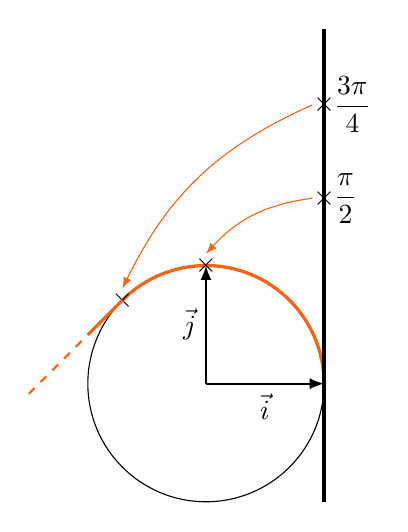
\begin{tikzpicture}[scale=1.5]
\draw [thick,->,>=latex] (0,0)--(0,1);
\draw [thick,->,>=latex] (0,0)--(1,0);
\draw (0,0.5) node[left] {$\vec{j}$};
\draw (0.5,0) node[below] {$\vec{i}$};
\draw (0,0) circle(1);
\draw [very thick,ocre] (1,0) arc (0:135:1);
\draw [very thick] (1,-1)--(1,3);
\draw (0,1) node {$\times$};
\draw (1,1.57) node {$\times$};
\draw (1,1.57) node[right] {$\dfrac{\pi}{2}$};
\draw [ocre, >=latex,->] (0.9,1.57)  to[bend right=20] (0,1.1);
\draw (1,2.36) node {$\times$};
\draw (-0.707,0.707) node {$\times$};
\draw (1,2.36) node[right] {$\dfrac{3\pi}{4}$};
\draw [ocre, >=latex,->] (0.9,2.36)  to[bend right=20] (-0.707,0.807);
\draw [very thick,ocre,domain=-1:-0.707] plot (\x,\x+1.414);
\draw [dashed, thick,ocre,domain=-1.5:-1] plot (\x,\x+1.414);
\end{tikzpicture}
\end{center}

\begin{proposition}
Deux réels dont la différence est le produit de $2\pi$ et d'un nombre entier ont la même image par $M$.
\end{proposition}
\subsection{Cosinus et sinus d'un nombre réel}

\begin{definition}
Soit $x$ un réel et $M(x)$ son image sur le cercle trigonométrique. On appelle :
\begin{itemize}
\item Cosinus de $x$, noté $\cos(x)$, l'abscisse de $M(x)$ ;
\item Sinus de $x$, noté $\sin(x)$, l'ordonnée de $M(x)$.
\end{itemize}
\end{definition}

\begin{center}
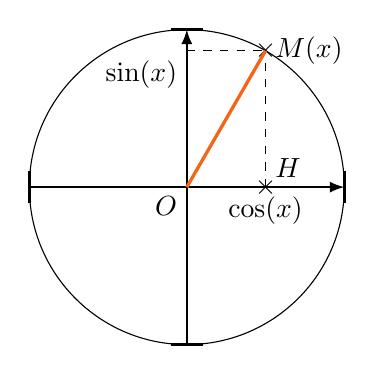
\begin{tikzpicture}[scale=2]
\draw [thick,->,>=latex] (0,-1)--(0,1);
\draw [thick,->,>=latex] (-1,0)--(1,0);
\draw (0,0) circle(1);
\draw (0.5,0.866) node {$\times$};
\draw (0.5,0.866) node[right] {$M(x)$};
\draw [dashed] (0.5,0)--(0.5,0.866);
\draw [dashed] (0,0.866)--(0.5,0.866);
\draw [very thick, ocre] (0,0)--(0.5,0.866);
\draw (0,0) node[below left] {$O$};
\draw (0.5,0) node[below] {$\cos(x)$};
\draw (0,0.866) node[below left] {$\sin (x)$};
\draw [very thick] (1,0.1) -- (1,-0.1);
\draw [very thick] (-1,0.1) -- (-1,-0.1);
\draw [very thick] (0.1,1) -- (-0.1,1);
\draw [very thick] (0.1,-1) -- (-0.1,-1);
\draw (0.5,0) node[above right] {$H$};
\draw (0.5,0) node {$\times$};
\end{tikzpicture}
\end{center}


\newpage 

\begin{example}On retiendra en particulier les valeurs remarquables suivantes.

\begin{center}
\renewcommand{\arraystretch}{2.5}
\noindent \begin{tabularx}{0.9\linewidth}{|X|XXXXXX|}
\hline
Degré & 0 & 30 & 45 & 60 & 90 & 180 \\
\hline
Radians & 0 & $\dfrac{\pi}{6}$ & $\dfrac{\pi}{4}$ & $\dfrac{\pi}{3}$ & $\dfrac{\pi}{2}$ & $\pi$ \\
\hline
Cosinus & 1 & $\dfrac{\sqrt{3}}{2}$ & $\dfrac{\sqrt{2}}{2}$ & $\dfrac{1}{2}$ & 0 & -1\\
\hline
Sinus & 0 & $\dfrac{1}{2}$ & $\dfrac{\sqrt{2}}{2}$ & $\dfrac{\sqrt{3}}{2}$ & 1 & 0\\
\hline
\end{tabularx}
\end{center}
\end{example}

\begin{center}

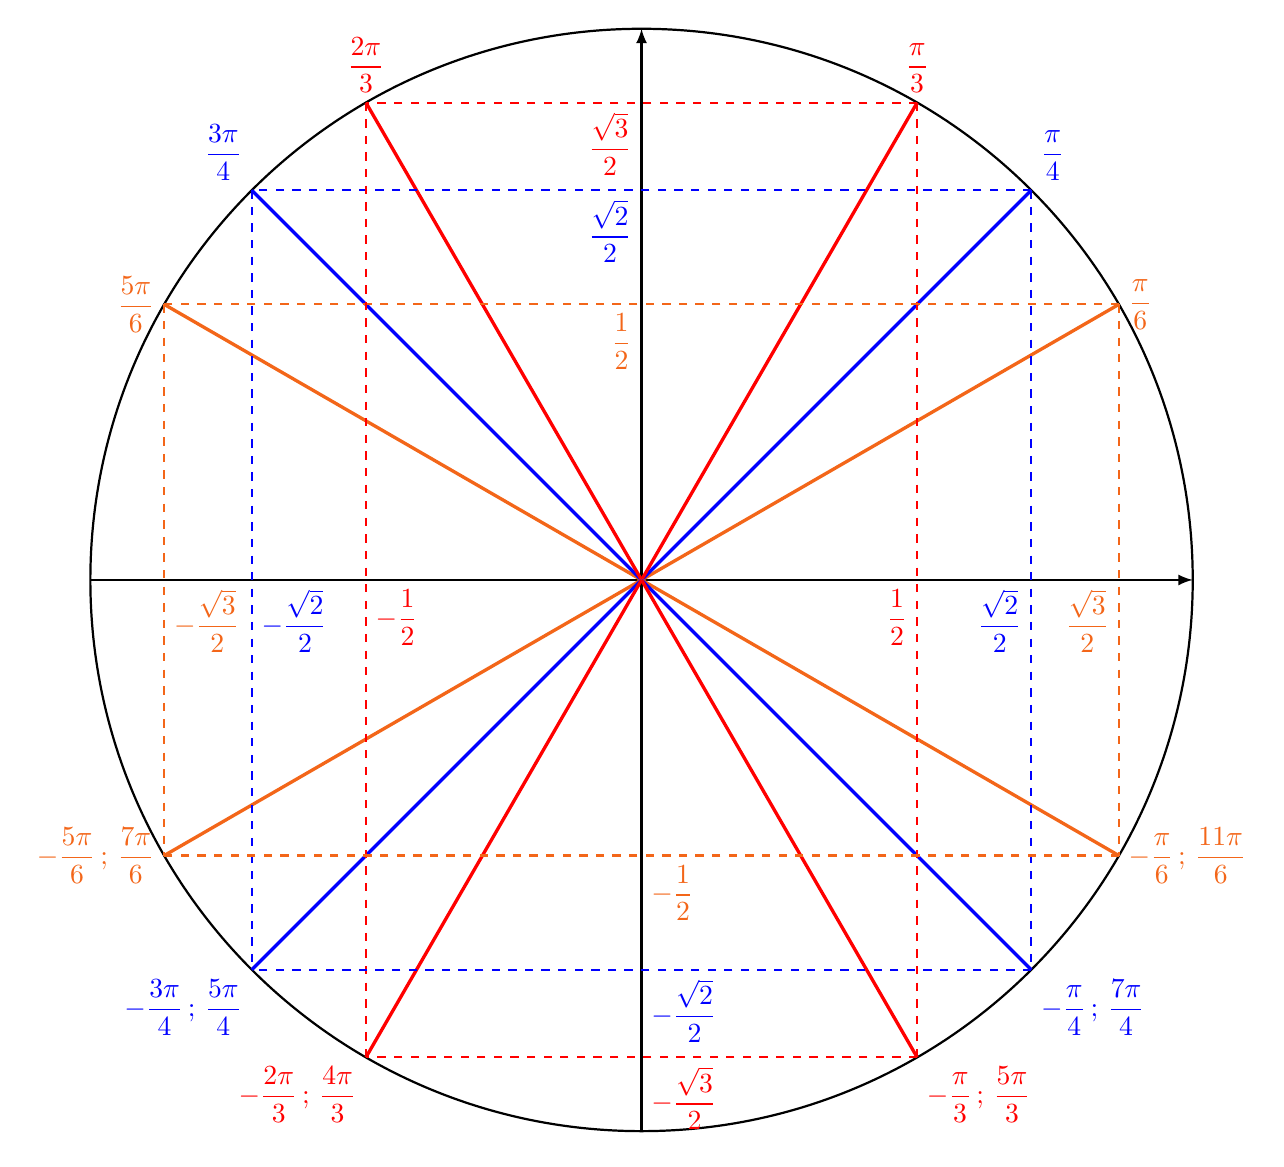
\begin{tikzpicture}[scale=7]
\draw [thick,>=latex,->] (0,-1) -- (0,1);
\draw [thick,>=latex,->] (-1,0) -- (1,0);
\draw [thick] (0,0) circle (1);
\draw [very thick, ocre] (0:0) -- (30:1);
\draw [very thick, blue] (0:0) -- (45:1);
\draw [very thick, red] (0:0) -- (60:1);
\draw [very thick, ocre] (0:0) -- (150:1);
\draw [very thick, blue] (0:0) -- (135:1);
\draw [very thick, red] (0:0) -- (120:1);
\draw [very thick, ocre] (0:0) -- (-30:1);
\draw [very thick, blue] (0:0) -- (-45:1);
\draw [very thick, red] (0:0) -- (-60:1);
\draw [very thick, ocre] (0:0) -- (-150:1);
\draw [very thick, blue] (0:0) -- (-135:1);
\draw [very thick, red] (0:0) -- (-120:1);
\draw [dashed,thick,red] (60:1) -- (-60:1);
\draw [dashed,thick,red] (60:1) -- (120:1);
\draw [dashed,thick,blue] (45:1) -- (-45:1);
\draw [dashed,thick,blue] (45:1) -- (135:1);
\draw [dashed,thick,ocre] (30:1) -- (-30:1);
\draw [dashed,thick,ocre] (30:1) -- (150:1);

\draw [dashed,thick,red] (120:1) -- (-120:1);
\draw [dashed,thick,red] (-60:1) -- (-120:1);
\draw [dashed,thick,blue] (135:1) -- (-135:1);
\draw [dashed,thick,blue] (-45:1) -- (-135:1);
\draw [dashed,thick,ocre] (150:1) -- (-150:1);
\draw [dashed,thick,ocre] (-30:1) -- (-150:1);

\draw [ocre] (0:0.866) node[below left] {$\dfrac{\sqrt{3}}{2}$};
\draw [blue] (0:0.707) node[below left] {$\dfrac{\sqrt{2}}{2}$};
\draw [red] (0:0.5) node[below left] {$\dfrac{1}{2}$};
\draw [red] (90:0.866) node[below left] {$\dfrac{\sqrt{3}}{2}$};
\draw [blue] (90:0.707) node[below left] {$\dfrac{\sqrt{2}}{2}$};
\draw [ocre] (90:0.5) node[below left] {$\dfrac{1}{2}$};

\draw [ocre] (180:0.866) node[below right] {$-\dfrac{\sqrt{3}}{2}$};
\draw [blue] (180:0.707) node[below right] {$-\dfrac{\sqrt{2}}{2}$};
\draw [red] (180:0.5) node[below right] {$-\dfrac{1}{2}$};
\draw [red] (-90:0.866) node[below right] {$-\dfrac{\sqrt{3}}{2}$};
\draw [blue] (-90:0.707) node[below right] {$-\dfrac{\sqrt{2}}{2}$};
\draw [ocre] (-90:0.5) node[below right] {$-\dfrac{1}{2}$};

\draw [ocre] (30:1) node[right] {$\dfrac{\pi}{6}$};
\draw [blue] (45:1) node[above right] {$\dfrac{\pi}{4}$};
\draw [red] (60:1) node[above] {$\dfrac{\pi}{3}$};
\draw [ocre] (150:1) node[left] {$\dfrac{5\pi}{6}$};
\draw [blue] (135:1) node[above left] {$\dfrac{3\pi}{4}$};
\draw [red] (120:1) node[above] {$\dfrac{2\pi}{3}$};

\draw [ocre] (-30:1) node[right] {$-\dfrac{\pi}{6}\, ; \, \dfrac{11\pi}{6}$};
\draw [blue] (-45:1) node[below right] {$-\dfrac{\pi}{4}\, ; \, \dfrac{7\pi}{4}$};
\draw [red] (-60:1) node[below right] {$-\dfrac{\pi}{3}\, ; \, \dfrac{5\pi}{3}$};
\draw [ocre] (-150:1) node[left] {$-\dfrac{5\pi}{6}\, ; \, \dfrac{7\pi}{6}$};
\draw [blue] (-135:1) node[below left] {$-\dfrac{3\pi}{4}\, ; \, \dfrac{5\pi}{4}$};
\draw [red] (-120:1) node[below left] {$-\dfrac{2\pi}{3}\, ; \, \dfrac{4\pi}{3}$};
\end{tikzpicture}
\newpage
\end{center}
\begin{proposition}
Pour tout réel $x$,
\[-1\leqslant \cos(x) \leqslant 1 \qquad -1\leqslant \sin(x) \leqslant 1 \qquad \cos(x)^2+\sin(x)^2=1\]
\vspace{-0.5cm}\end{proposition}


\begin{example}On considère la fonction $f:x \mapsto \dfrac{1+x}{2+\sin(x)}$.

Puisque, pour tout $x\in\mathbb{R}$, $1 \geqslant \sin(x) \geqslant -1$, alors $3 \geqslant 2+\sin(x)\geqslant 1 >0$. $f$ est donc bien définie sur $\mathbb{R}$. 

Par ailleurs, la fonction inverse étant décroissante sur $]0;+\infty [$, on a $\dfrac{1}{3} \leqslant \dfrac{1}{2+\sin(x)}\leqslant 1$ et donc, en multipliant par $1+x$ qui est strictement positif sur $]0;+\infty[$, $\dfrac{1+x}{3}\leqslant f(x)$. 

Or, $\displaystyle\lim_{x\to + \infty} \left(\dfrac{1+x}{3}\right)=+\infty$. Par comparaison, $\displaystyle\lim_{x\to +\infty}f(x)=+\infty$.\end{example}


\subsection{Résolution d'équation et d'inéquation}

\begin{example}Les solutions de l'équation $\cos(x)=\dfrac{1}{2}$ sur $[-\pi;\pi]$ sont $-\dfrac{\pi}{3}$ et $\dfrac{\pi}{3}$.\end{example}

\begin{example}Le solutions de l'équation $\cos(x)=0$ sur $[0;2\pi]$ sont $\dfrac{\pi}{2}$ et $\dfrac{3\pi}{2}$.\end{example}



\begin{example}L'ensemble des solutions de l'inéquation $\cos(x) \leqslant \dfrac{\sqrt{3}}{2}$ sur $[0;2\pi]$ est l'intervalle $\left[ \dfrac{\pi}{6};\dfrac{11\pi}{6}\right]$.

Sur l'intervalle $[-\pi;\pi]$ l'ensemble des solutions de cette inéquation est $\left[-\pi; -\dfrac{\pi}{6}\right]\cup\left[\dfrac{\pi}{6};\pi\right]$.\end{example}



\begin{center}

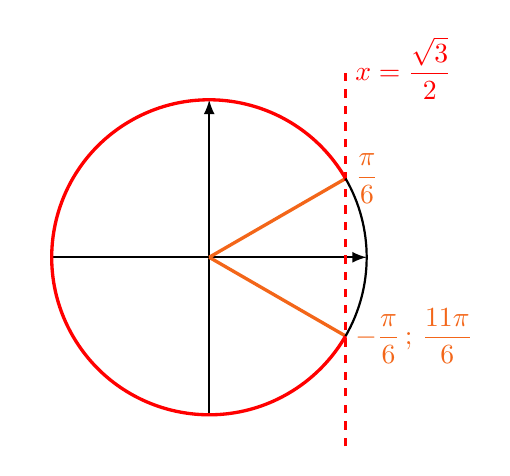
\begin{tikzpicture}[scale=2]
\draw [thick,>=latex,->] (0,-1) -- (0,1);
\draw [thick,>=latex,->] (-1,0) -- (1,0);
\draw [very thick, ocre] (0:0) -- (30:1);
\draw [very thick, ocre] (0:0) -- (-30:1);
\draw [dashed,thick,red] (0.866,-1.2) -- (0.866,1.2);

\draw [red] (0.866,1.2) node[right] {$x=\dfrac{\sqrt{3}}{2}$};
\draw [very thick, red] (30:1) arc (30:330:1);
\draw [ thick, black] (-30:1) arc (-30:30:1);

\draw [ocre] (30:1) node[right] {$\dfrac{\pi}{6}$};

\draw [ocre] (-30:1) node[right] {$-\dfrac{\pi}{6}\, ; \, \dfrac{11\pi}{6}$};

\end{tikzpicture}\end{center}

Il faut donc faire attention à l'intervalle de résolution.. Dans tous les cas, le cercle trigonométrique sera votre plus précieux allié.
\newpage 
\section{Fonctions trigonométriques}

\subsection{Définition et variations}

\begin{definition}
La fonction cosinus est la fonction qui, à tout réel $x$, associe $\cos (x)$.\\
La fonction sinus est la fonction qui, à tout réel $x$, associe $\sin (x)$.\\
\end{definition}

\begin{center}
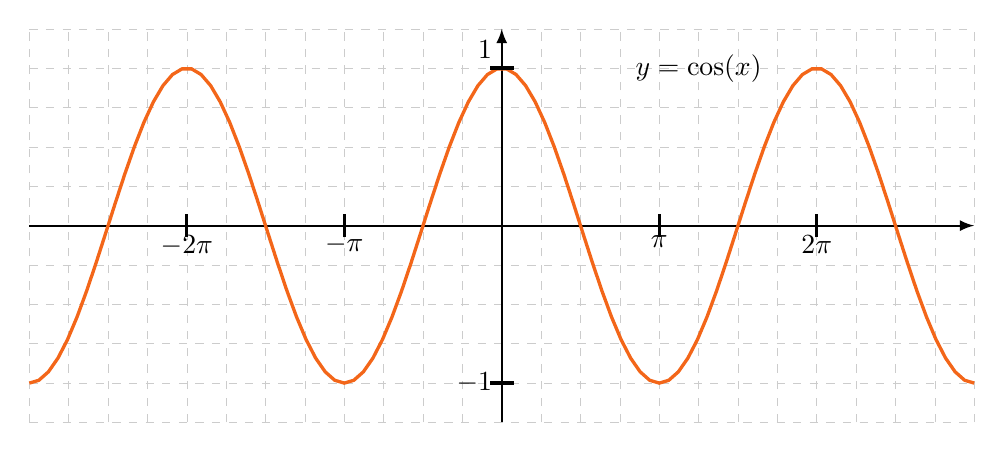
\begin{tikzpicture}[scale=0.5]
\draw [dashed, very thin, gray!40] (-12,-5) grid (12,5);
\draw [>=latex,->,thick] (-12,0) -- (12,0);
\draw [>=latex,->,thick] (0,-5) -- (0,5);
\draw [ocre, very thick,samples=100,domain=-12:12] plot (\x, {4*cos(pi*\x/4 r)}); 
\draw [very thick] (4,-0.3) -- (4,0.3);
\draw [very thick] (8,-0.3) -- (8,0.3);
\draw [very thick] (-4,-0.3) -- (-4,0.3);
\draw [very thick] (-8,-0.3) -- (-8,0.3);
\draw [very thick] (0.3,4) -- (-0.3,4);
\draw [very thick] (0.3,-4) -- (-0.3,-4);
\draw (4,0) node[below] {$\pi$};
\draw (-4,0) node[below] {$-\pi$};
\draw (8,0) node[below] {$2\pi$};
\draw (-8,0) node[below] {$-2\pi$};
\draw (0,4) node[above left] {$1$};
\draw (0,-4) node[left] {$-1$};
\draw (5,4) node {$y=\cos (x)$};
\end{tikzpicture}
\end{center}

\begin{center}
  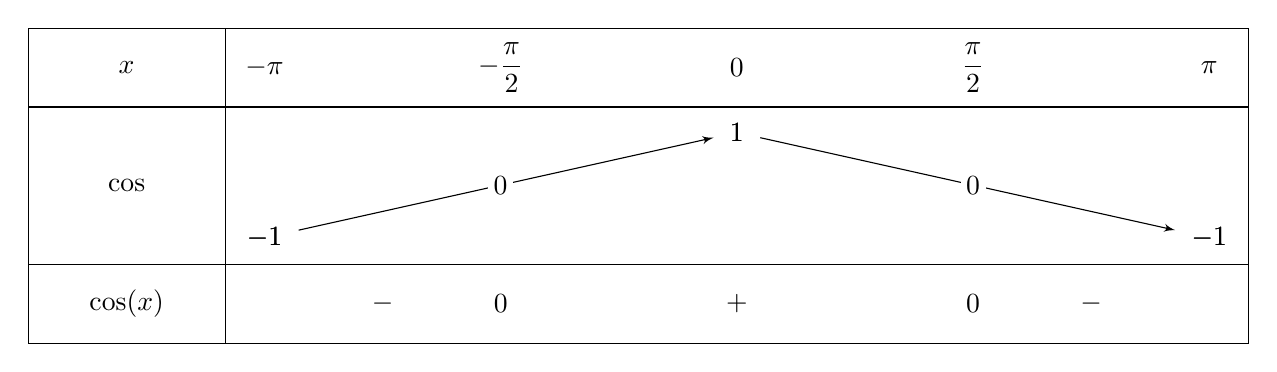
\begin{tikzpicture}[scale=1]
  \tikzset{node style/.style = {inner sep = 2pt, outer sep = 2pt}}
   \tkzTabInit[lgt=2.5]{$x$ / 1 , $\cos$ / 2,$\cos(x)$ / 1}{$-\pi$,$-\dfrac{\pi}{2}$,$0$,$\dfrac{\pi}{2}$, $\pi$}

   \tkzTabVar{-/$-1$,R,+/$1$,R,-/$-1$}
   \tkzTabIma{1}{3}{2}{0}
   \tkzTabIma{3}{5}{4}{0}
   \tkzTabLine{,-,0,,+,,0,- }
     
      
   \end{tikzpicture}  
\end{center}

\begin{center}
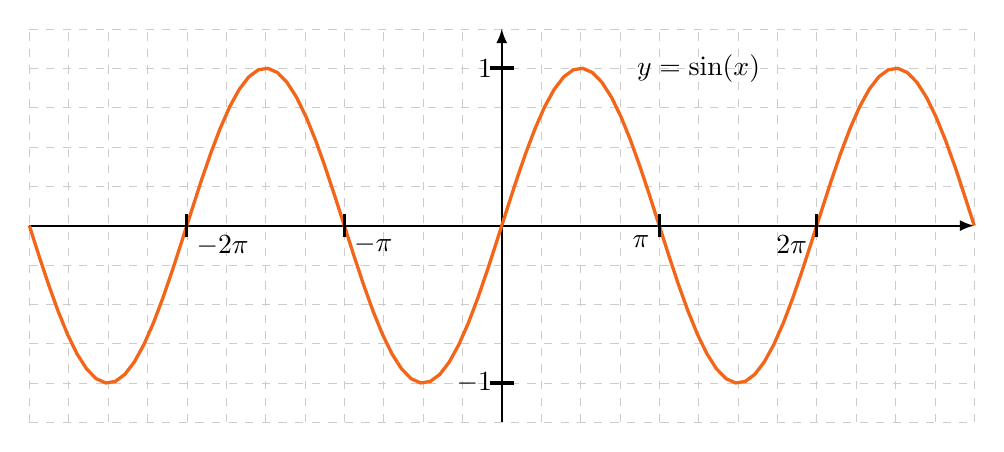
\begin{tikzpicture}[scale=0.5]
\draw [dashed, very thin, gray!40] (-12,-5) grid (12,5);
\draw [>=latex,->,thick] (-12,0) -- (12,0);
\draw [>=latex,->,thick] (0,-5) -- (0,5);
\draw [ocre, very thick,samples=100,domain=-12:12] plot (\x, {4*sin(pi*\x/4 r)}); 
\draw [very thick] (4,-0.3) -- (4,0.3);
\draw [very thick] (8,-0.3) -- (8,0.3);
\draw [very thick] (-4,-0.3) -- (-4,0.3);
\draw [very thick] (-8,-0.3) -- (-8,0.3);
\draw [very thick] (0.3,4) -- (-0.3,4);
\draw [very thick] (0.3,-4) -- (-0.3,-4);
\draw (4,0) node[below left] {$\pi$};
\draw (-4,0) node[below right] {$-\pi$};
\draw (8,0) node[below left] {$2\pi$};
\draw (-8,0) node[below right] {$-2\pi$};
\draw (0,4) node[left] {$1$};
\draw (0,-4) node[left] {$-1$};
\draw (5,4) node {$y=\sin (x)$};
\end{tikzpicture}
\end{center}

\begin{center}
  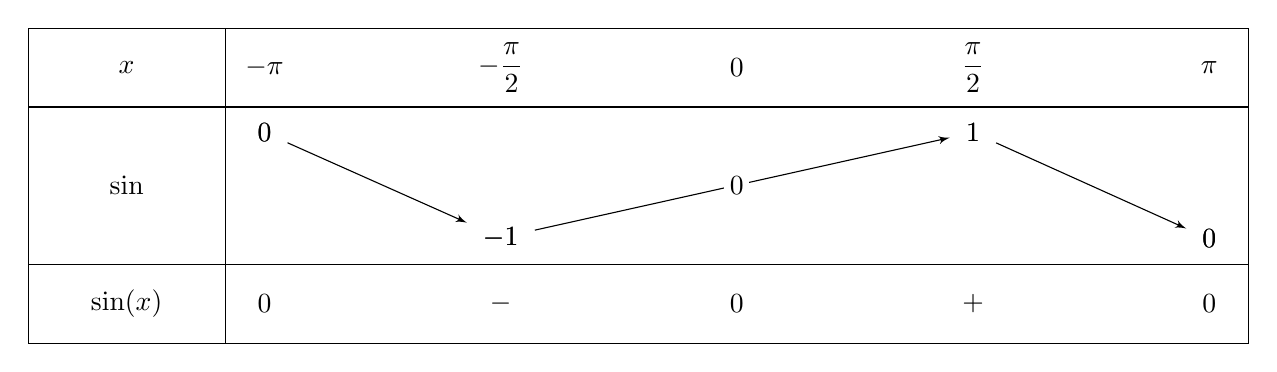
\begin{tikzpicture}[scale=1]
  \tikzset{node style/.style = {inner sep = 2pt, outer sep = 2pt}}
   \tkzTabInit[lgt=2.5]{$x$ / 1 , $\sin$ / 2,$\sin(x)$ / 1}{$-\pi$,$-\dfrac{\pi}{2}$,$0$,$\dfrac{\pi}{2}$, $\pi$}

   \tkzTabVar{+/$0$,-/$-1$,R,+/$1$,-/$0$}
   \tkzTabIma{2}{4}{3}{0}
   \tkzTabLine{0,,-,,0,,+,,0 }
     
      
   \end{tikzpicture}  
\end{center}

\begin{proposition}
Pour tout $x \in \mathbb{R}$, on a
\begin{itemize}
\item $\cos(-x)=\cos (x)$, la fonction cosinus est paire.
\item $\sin (-x)= -\sin (x)$; la fonction sinus est impaire.
\end{itemize}
\vspace{-0.5cm}\end{proposition}

Cela se traduit graphiquement par le fait que la courbe de la fonction cosinus est symétrique par rapport à l'axe des ordonnées alors que la courbe de la fonction sinus est symétrique par rapport à l'origine du repère.

\begin{example}
$\cos \left( -\dfrac{\pi}{4} \right) = \cos \left( \dfrac{\pi}{4} \right)= \dfrac{\sqrt{2}}{2}\qquad ; \qquad \sin \left( -\dfrac{\pi}{4} \right) = -\sin \left( \dfrac{\pi}{4} \right)= -\dfrac{\sqrt{2}}{2}$ .
\end{example}

\begin{proposition}Pour tout $x\in\mathbb{R}$ et pour tout $k\in\mathbb{Z}$, on a
\begin{itemize}
\item $\cos (x+k\times 2\pi)=\cos (x)$ ;
\item $\sin (x+k\times 2\pi) = \sin (x)$.
\end{itemize}
On dit que les fonctions sinus et cosinus sont $2\pi$-périodiques. \end{proposition}

\begin{example}
$\cos \left( \dfrac{25\pi}{3}\right)= \cos \left( \dfrac{24\pi}{3}+\dfrac{\pi}{3}\right)=\cos \left(4\times 2\pi + \dfrac{\pi}{3}\right)=\cos\left( \dfrac{\pi}{3}\right)=\dfrac{1}{2}$.
\end{example}

\subsection{Dérivée des fonctions trigonométriques}

\begin{proposition}Les fonctions $\cos$ et $\sin$ sont dérivables sur $\mathbb{R}$. Par ailleurs, pour tout réel $x$,
\[\sin'(x)=\cos(x) \qquad \text{et}\qquad \cos'(x)=-\sin(x)\]
\vspace{-0.5cm}\end{proposition}

\begin{example}On considère la fonction $g: x\mapsto 2\cos(x)-x$ définie sur $I=[-\pi;\pi]$. $g$ est dérivable sur $I$ et pour tout $x\in I$, $g'(x)=-2\sin(x)-1$. 

Ainsi, $g'(x)\geqslant 0$ si et seulement si $\sin(x) \leqslant -\dfrac{1}{2}$. 

Pour résoudre cette inéquation on peut utiliser le cercle trigonométrique.

\begin{minipage}{0.6\linewidth}

Ainsi, $g'(x)\geqslant 0$ si et seulement si $\sin(x) \leqslant -\dfrac{1}{2}$. 

Pour résoudre cette inéquation on peut utiliser le cercle trigonométrique.

L'ensemble des solutions de l'inéquation $\sin(x) \leqslant -\dfrac{1}{2}$ sur $[-\pi;\pi]$ est $\left[-\dfrac{5\pi}{6};-\dfrac{\pi}{6}\right]$. On peut alors construire le tableau de variations de $f$ sur l'intervalle $[-\pi;\pi]$

\end{minipage}\hfill \begin{minipage}{0.35 \linewidth}
\begin{center}
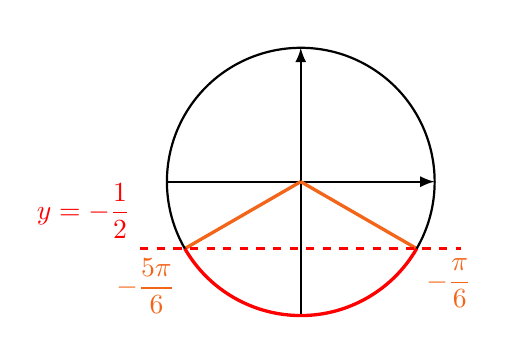
\begin{tikzpicture}[scale=1.7]
\draw [thick,>=latex,->] (0,-1) -- (0,1);
\draw [thick,>=latex,->] (-1,0) -- (1,0);
\draw [very thick, ocre] (0:0) -- (-150:1);
\draw [very thick, ocre] (0:0) -- (-30:1);
\draw [dashed,thick,red] (-1.2,-0.5) -- (1.2,-0.5);

\draw [red] (-1.2,-0.5) node[above left] {$y=-\dfrac{1}{2}$};
\draw [very thick, red] (-150:1) arc (-150:-30:1);
\draw [ thick, black] (-30:1) arc (-30:210:1);

\draw [ocre] (-150:1) node[below left] {$-\dfrac{5\pi}{6}$};

\draw [ocre] (-30:1) node[below right] {$-\dfrac{\pi}{6}$};

\end{tikzpicture}\end{center}
\end{minipage}


\begin{center}
  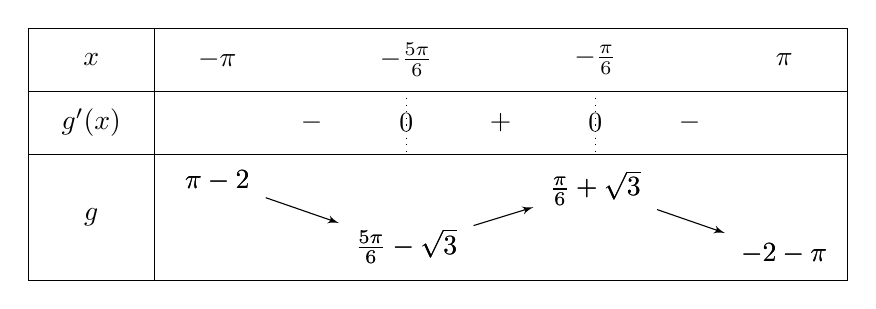
\begin{tikzpicture}[scale=0.8]
  \tikzset{node style/.style = {inner sep = 2pt, outer sep = 2pt}}
   \tkzTabInit[espcl=3, deltacl = 1]{$x$ / 1 , $g'(x)$ / 1,$g$ / 2}{$-\pi$,$-\frac{5\pi}{6}$,$-\frac{\pi}{6}$, $\pi$}
	\tkzTabLine{,-,z,+,z,-, }
   \tkzTabVar{+/$\pi-2$,-/$\frac{5\pi}{6}-\sqrt{3}$,+/$\frac{\pi}{6}+\sqrt{3}$,-/$-2-\pi$}
  \end{tikzpicture}  
\end{center}
\vspace{-1cm}

\end{example}


Il est également possible de dérivée des fonctions composées avec le cosinus ou le sinus.
\begin{proposition}Soit $u$ une fonction définie et dérivable sur un intervalle $I$. Alors $\sin (u)$ et $\cos(u)$ sont également dérivables sur cet intervalle $I$ et on a
\[(\sin(u))'=u'\times \cos(u) \qquad \text{et}\qquad (\cos(u))'=-u'\times \sin(u)\]
\vspace{-0.5cm}\end{proposition}



\begin{example}Pour tout réel $x$, on pose $f(x)=\sin(3x^2-4x+5)$. 

$f$ est dérivable sur $\mathbb{R}$ et pour tout réel $x$, $f'(x)=(6x-4)\sin(3x^2-4x+5)$.\end{example}

\begin{proposition}Soit $a$ un réel non nul.
\begin{itemize}
\item Une primitive de $x\mapsto \cos(ax)$ sur $\mathbb{R}$ est $x\mapsto \dfrac{\sin(ax)}{a}$.
\item Une primitive de $x\mapsto \sin(ax)$ sur $\mathbb{R}$ est $x\mapsto -\dfrac{\cos(ax)}{a}$.
\end{itemize}\end{proposition}

\begin{demonstration}Il suffit de dériver. Attention au signe !\end{demonstration}

\begin{example}Pour tout réel $x$, on pose $f(x)=3\cos(2x)-5\sin(9x)$.
Une primitive de $f$ sur $\mathbb{R}$ est la fonction $F$ définie pour tout réel $x$ par $F(x)=\dfrac{3}{2}\sin(2x)+\dfrac{5}{9}\cos(9x)$.\end{example}

\begin{example}Pour $x\in\mathbb{R}$, on pose $g(x)=\cos(x)\sin(x)$. Pour tout $x\in\mathbb{R}$, on a $g(x)=\sin'(x) \times \sin (x)$. 

Une primitive de $g$ sur $\mathbb{R}$ est la fonction $G$ définie pour tout réel $x$ par $G(x)=\dfrac{1}{2}\sin^2(x)$.\end{example}

\begin{example}On considère la fonction $f:x\mapsto \sin^3(x)\dx$ définie sur $\mathbb{R}$ et $I=\displaystyle\int_0^{\pi} f(x)\dx$.

D'une part, pour tout réel $x$,
\[f(x)=\sin(x) \times \sin^2(x) = \sin(x)(1-\cos^2(x))=\sin(x)-\sin(x)\cos^2(x).\]
Ainsi, $I = \displaystyle\int_0^{\pi}\sin(x)\dx+\displaystyle\int_0^{\pi}(-\sin(x)\cos^2(x))\dx$. D'une part, 
\[\displaystyle\int_0^{\pi}\sin(x)\dx = [-\cos(x)]_0^{\pi}=-\cos(\pi)-(-\cos(0))=-(-1)-(-1)=2.\]
D'autre part, pour tout réel $x\in[0;\pi]$, on a $-\sin(x)\cos^2(x)=\cos'(x) \times \cos^2(x)$. \\Une primitive de la fonction $x\mapsto -\sin(x)\cos^2(x)$ sur $[0;\pi]$ est donc la fonction $x\mapsto \dfrac{\cos^3(x)}{3}$. Ainsi,
\[\displaystyle\int_0^{\pi}(-\sin(x)\cos^2(x))\dx=\left[\dfrac{\cos^3(x)}{3}\right]_{0}^{\pi}=\dfrac{\cos^3(\pi)}{3}-\dfrac{\cos^3(0)}{3}=-\dfrac{1}{3}-\dfrac{1}{3}=-\dfrac{2}{3}.\]
Finalement, $I=2-\dfrac{2}{3}=\dfrac{4}{3}$.\end{example}




\end{document}